\documentclass[tikz]{standalone}
\usepackage{thesis}

\begin{document}
\newcommand{\spinup}{\tikz\draw[spin] (0,-1ex) -- (0, 1ex);}
\newcommand{\spindn}{\tikz\draw[spin] (0, 1ex) -- (0,-1ex);}
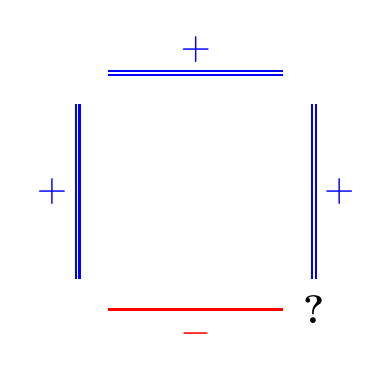
\begin{tikzpicture}[
  scale=3,
  spin/.style={-latex, very thick},
  site/.style={inner sep=0, minimum size=5ex},
  fm/.style={blue,double},
  afm/.style={red},
  every node/.style={font=\Large},
  every edge/.append style={thick}
]
  \node [site] (1) at (1,1) {\spinup};
  \node [site] (2) at (0,1) {\spinup} edge[fm] node[above] {$+$} (1);
  \node [site] (3) at (0,0) {\spinup} edge[fm] node[left]  {$+$} (2);
  \node [site] (4) at (1,0) {\textbf{?}}
    edge[afm] node[below] {$-$} (3)
    edge[fm]  node[right] {$+$} (1);
\end{tikzpicture}
\end{document}
